\documentclass[a4paper]{article}
\usepackage[mac]{inputenc}
\usepackage{xcolor}
\usepackage{graphicx}
\usepackage{amssymb}
\usepackage{a4wide}
\usepackage{stringstrings}
\usepackage{titling}
\usepackage[pdftex,colorlinks=true,pdfstartview=FitV,linkcolor=black,citecolor= black,urlcolor= black]{hyperref}
%%%%%%%%%%%%%%%%%%%%%%%%%%%%%%%%%%%%%%%%%%%%%%%%%%%%%%%%%%%%
\usepackage{ifthen}
\usepackage{fancyhdr}

\newboolean{longversion}
\setboolean{longversion}{false} % toggle for long/short version
% \setboolean{longversion}{true} % toggle for long/short version
\ifthenelse{\boolean{longversion}}
{
	\newcommand{\longcv}[1]{#1}
	\newcommand{\shortcv}[1]{}
}{
	\newcommand{\longcv}[1]{}
	\newcommand{\shortcv}[1]{#1}
}
% \newcommand{\period}{(since 2007)}
\renewcommand{\labelitemi}{---}% {$\bullet$}

\newcommand{\nbc}[3]{
 {\colorbox{#3}{\bfseries\sffamily\scriptsize\textcolor{white}{#1}}}
 {\textcolor{#3}{\sf\small$\blacktriangleright$\textit{#2}$\blacktriangleleft$}}}
\newcommand\ml[1]{\nbc{ML}{#1}{violet}} % add more author macros here

%%%%%%%%%%%%%%%%%%%%%%%%%%%%%%%%%%%%%%%%%%%%%%%%%%%%%%%%%%%%
\pdfinfo{
  /Title(Curriculum Vitae)
  /Author(Mircea F. Lungu)
  /Subject()
  /Keywords($Id$)
}
%%%%%%%%%%%%%%%%%%%%%%%%%%%%%%%%%%%%%%%%%%%%%%%%%%%%%%%%%%%%
\begin{document}
\longcv{\title{\textsf{Mircea F. Lungu, PhD \\Curriculum Vit\ae}}}
\shortcv{\title{\textsf{Mircea F. Lungu, PhD \\Curriculum Vit\ae}}}


\pagestyle{myheadings}
\pagestyle{fancy}

\thispagestyle{plain}

% \markright{Mircea F. Lungu --- CV --- \today}
\renewcommand{\headrulewidth}{0.0pt}
\renewcommand{\footrulewidth}{0.0pt}

\lfoot{M.F. Lungu, CV}

\posttitle{\par\end{center}\vspace{-0.8cm}}
\date{\small http://mir.lu/cv}
\maketitle

\thispagestyle{empty}


%%%%%%%%%%%%%%%%%%%%%%%%%%%%%%%%%%%%%%%%%%%%%%%%%%%%%%%%%%%%

% \vspace{-4cm}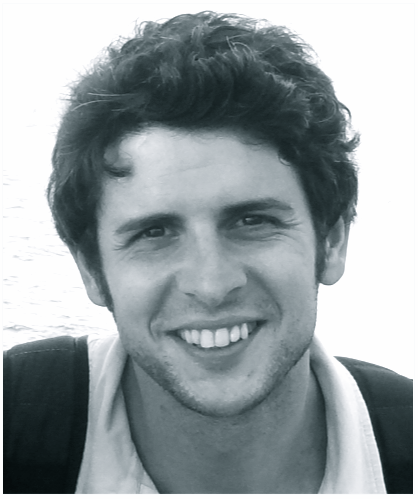
\includegraphics[width=3cm]{ml-bw.png}
% \vspace{0.5cm}


\newcommand{\cvsection}[1]{\section*{\capitalizetitle{#1}}\vspace{-0.75em}\hrule\vspace{1em}}


% Empirical Software Engineering, 
% Software evolution,
% Reverse and re-engineering,
% Programming Languages,
% Triathlon, Music, Theatre.


\newcommand{\degree}[5]{#2 & {\bf #1}\\ & #3\\ &#4\\ &#5\\ \\}
%%%%%%%%%%%%%%%%%%%%%%%%%%%%%%%%%%%%%%%%%%%%%%%%%%%%%%%%%%%%
\cvsection{Education}

\begin{tabular}{p{3cm} p{11cm}}

\degree
	{PhD}
	{2009}
	{Faculty of Informatics, University of Lugano}
	{Dissertation: {\em Reverse Engineering Software Ecosystems}}
	{Advisor: Prof. Dr. Michele Lanza}

\degree
	{Dipl. -Ing.}
	{2004}
	{Computer Science Department, Polytechnic University of Timisoara}
	{Thesis: \emph{Conformity Strategies - Measures of Software Design Rules}}
	{Supervisor: Prof. Dr. Radu Marinescu}

\end{tabular}

\newcommand{\job}[4]{#1 & {\bf #3}\\ & #2\\  &{\em#4}\\ \\}
%%%%%%%%%%%%%%%%%%%%%%%%%%%%%%%%%%%%%%%%%%%%%%%%%%%%%%%%%%%%
\cvsection{Experience}

\begin{tabular}{r p{8cm}}

	\job
	{Aug 2010 -- present}
	{Computer Science Institute, University of Bern}
	{Researcher \& Lecturer}
	{
	%Assisting Oscar Nierstrasz in managing the SCG. 
	Conducting research in software engineering and programming languages. Mentoring graduate students. Teaching a variety of lectures.}

	\job
	{2009 -- 2010}
	{Faculty of Informatics, University of Lugano}
	{Postdoctoral Researcher}
	{Conducting research in software evolution.}

	\job 
	{Jul -- Dec, 2007}
	{IBM TJ Watson Research Center, NY}
	{Visiting Researcher}
	{Visualizing distributed systems with Wim De Pauw}


	\job 
	{2004 -- 2009}
	{Faculty of Informatics, University of Lugano}
	{PhD Student}
	{Conducting research in software evolution, visualization, and large scale software analysis}


	\job
	{2001 -- 2003}
	{Computervoice Systems, Timisoara, RO}
	{Software Engineer}
	{Writing customer management software for several telecommunication companies from the US}

	\job
	{1999 -- 2001}
	{Logos Professional Highschool, Timisoara, RO}
	{Instructor}
	{Teaching Introduction to Programming with Pascal}

\end{tabular}
% ==========================================================



% ==========================================================


%%%%%%%%%%%%%%%%%%%%%%%%%%%%%%%%%%%%%%%%%%%%%%%%%%%%%%%%%%%%
\cvsection{Funded Research Projects}
\begin{tabular}{p{15cm}}
	Agile Software Assessment is a project funded by the Swiss National Science Foundation (SNSF project \# 200020-144126/1). Funding:	650,000.� SFr. Period:	Jan 1, 2013 - Dec. 30, 2015
\end{tabular}


%!TEX root = resume-long.tex
\newcommand {\conf}[3]{ $^{ #2}$ #1  & #3  \\}
\newcommand {\activity}[4]{$^{ #2}$ #1  & #3 \\ & {\em \small #4} \vspace {0.5em}\\}
\newcommand {\event}[4]{\activity{#1}{#2}{#3}{#4}}


\newcommand {\track}[1]{ \emph{(#1)}}
\newcommand {\tdtrack}{\track{TD} }
\newcommand {\eratrack}{\track{ERA} }
\newcommand {\tderatrack}{\track{TD,ERA} }
\newcommand {\tablesection}[1]{\\ \\ & \multicolumn{1}{l}{\bf  #1} \vspace{0.5em}\\}
\newcommand {\contrib}[1]{\hspace{1em} #1\\}


\cvsection{Professional Activities (Selected)}
% Corresponding years are superscripted where available.

\begin{tabular}{rp{10.4cm}}


\tablesection{Project Writer}

	\conf{ASA}{`13}{\href{http://p3.snf.ch/Project-144126}{Agile Software Assessment} -- project co-written with Oscar Nierstrasz funded by the Swiss NSF (project \# 200020-144126/1)}


\tablesection{External Expert}

	\conf{NWO}{}{Netherlands Organization for Scientific Research}
	\conf{EU}{}{European Commission's FP7 Programme}


\tablesection{Program Chair}

	\conf{VISSOFT}{`14}
	{IEEE Working Conference on Software Visualization \eratrack}

	\conf{CSMR}{`12}
	{European Conference on Maintenance \& Reengineering \tdtrack}

	\conf{WCRE}{`11}
	{International Conference on Reverse Engineering \tdtrack}

\tablesection{Co-Organizer}
 
	\event
		{CHOOSE Forum}
		{`12, `13, `14}
		{Yearly event that brings together the SE Industry and Research}
		{with Tudor Girba and Michele Lanza (University of Lugano)}

	\event
		{WEA}{`13, `14} 
		{International Workshop on Software Ecosystem Architectures}
		{with Jens Knodel (Fraunhofer Institute)}

	\event
		{SATTOSE}{`13} 
		{Seminar on Advanced Techniques in Software Engineering}
		{with Oscar Nierstrasz (University of Bern)}

	\event
		{USI PhD Talks}{`06 - `09}
		{Weekly interdisciplinary research presentations}
		{with Cyrus Hall}


\tablesection{Journal Reviewer}

	\conf{TSE}{}{IEEE Transactions on Software Engineering} % 2014

	\conf{JSME}{}{Software Maintenance and Evolution} % 2012 

	\conf{EMSE}{}{Empirical Software Engineering}

	\conf{JSS,SCP}{}{Elsevier: Systems and Software, Science of Computer Programming}

	% \conf{SCP}{}{Elsevier }

	% \conf{FTHCI}{}{Foundations and Trends in Human Computer Interaction}

	\conf{IEEE Software}{}{The IEEE Software Magazine}
 



\tablesection{Conference PC Member}

	\conf{SANER}{`15}{22nd Int. Conf. on Software Analysis, Evolution and Reengineering}

	\conf{OOPSLA}{`13}{Conference on Systems, Programming, Languages and Applications}

	\conf{ICSE}{`12, `14}{Int. Conf.  on Software Engineering \tdtrack}

	\conf {ICPC}{`14}{Int. Conf.  on Program Comprehension}

	\conf{WCRE}{`12, `13, `14}{Int. Conf.  on Reverse Engineering}

	\conf{ICSME}{`11, `12, `14}{Int. Conf. on Software Maintenance \& Evolution\tderatrack}


	\conf{MSR}{`14, 15}{Int. Conf. om Mining Software Repositories}
	% \conf{WASDeTT}{`11, `13}{Workshop on Advanced Software Development Tools and Techniques}

	\conf{ESEC/FSE}{`11}{European Software Engineering/ACM SIGSOFT Symposium on the Foundations of Software \tdtrack}


% \end{tabular}
% 2014 & WCRE + CSMR, ICSE (TD Track)\\
% 2013 & OOPSLA, WCRE, WASDeTT, CSMR, ICSM (TD Track) \\
% 2012 & ICSE (Posters \& TD Track), WCRE, ICSM (TD Track), CSMR \\
% 2011 & ICSM (TD Track), WASDeTT, ESEC/FSE 2011 (TD Track), CSMR, IWPSE/EVOL\\
% 2010 & IWSECO, WSE\\





\end{tabular}






% \subsubsection*{Member Of Professional Organizations}
% CHOOSE - Swiss Group for Object Oriented Systems and Environments \footnote{\url{http://choose.s-i.ch}} 2011 - present.



\newpage
%!TEX root = resume-long.tex

\cvsection{Honours and Awards (Selected)}
\newcommand {\award}[3]{\makebox[3.5cm][r]{\small #3} & {\bf #1} \\ & #2 \vspace{0.7em}\\}

\begin{tabular}{rp{10.5cm}}

	\award
		{OOPSLA Best Reviewer Award}
		{The ACM SIGPLAN Conference on Systems, Programming, Languages and Applications}
		{2013}

	\award 
		{Vice-President of CHOOSE}
		{The Swiss Group for Object Oriented Systems and Environments}
		{}

	\award
		{Best Paper Award}
		{With Lile Hattori at IWPSE-EVOL 2010 for {\em Replaying Past Changes in Multi-Developer Projects}}
		{2010}

	\award
		{1st Place}
		{ESUG Innovation Awards for the {\em Small Project Observatory} a platform for the visualization, monitoring, and analysis of software ecosystems}
		{2007}

	% \award
	% 	{Best Poster Award}
	% 	{The 3rd International ACM Symposium on Software Visualization, Brighton 2006, for the poster {\em Cutting Edge Software Visualization}}
	% 	{2006}

	\award
		{Best Software Engineer Award}
		{The Software Engineering Project at the Polytechnic University of Timisoara, RO}
		{2003}

	\award
		{2nd Place}
		{With {\em UPT} for building an image processing-based security system in 48 hours International {\em Hard \& Soft} Competition, Suceava, RO}
		{2002}

	% \award
	% 	{3rd Place}
	% 	{The National Student Software Development Contest, Focsani, RO}
	% 	{1999}

\end{tabular}




%


%!TEX root = CV_Publist_MirceaLungu.tex

\cvsection{Invited Talks}
Conference presentations are not included.
\vspace{1em}

\newcommand {\talk}[4]{\makebox[3cm][r]{\small #4} & {\bf #1} \\ & #3 (#2) \vspace{0.75em} \\}

\begin{tabular}{rp{10.5cm}}
	
	\talk 
		{Program Comprehension Across Levels of Abstraction}
		{Invited Talk}
		{University of California, Irvine}
		{May, 2013}

	\talk
		{Software is Data Too}
		{Keynote}
		{Smalltalks 2012, Argentina}
		{Nov, 2012}

	\talk
		{What do I talk about when I talk about Software Ecosystems}
		{Invited Talk}
		{University of Buenos Aires}
		{}	

	\talk 
		{Reverse Engineering Software Ecosystems}
		{Invited Talk}
		{University of California, Irvine}
		{Jul, 2011}

	\talk
		{Ecosystem Analysis}
		{Invited Talk}
		{PL'10: The 3$^{rd}$ Summer School on Programming Languages}
		{Nov, 2010}

	\talk
		{Architecture Recovery}
		{Guest Lecture}
		{University of Lugano}
		{Sep, 2010}

	\talk
		{Web-based visualization tools for reverse engineering}
		{Invited Talk}
		{2nd International Workshop on Advanced Software Development Tools and Techniques, Beijing}
		{Oct 2008}

	\talk 
		{The Small Project Observatory}
		{Invited Talk}
		{IBM TJ Watson Research Center}
		{Nov, 2007}
\end{tabular}



% \newcommand {\lecture}[3]{{\small #3} & {\bf #1} \\ & #2 \vspace{0.7em}\\ }
\newcommand {\lecture}[3]{\item {\em #1}\\#2, #3 }
\newcommand {\ub}{University of Bern}
\newcommand {\ul}{University of Lugano}
\newcommand {\msc}{MSc, }
\newcommand {\bsc}{BSc, }

\cvsection{Lecturing}
\begin{enumerate}
	\lecture{Software Engineering}{\bsc \ub}{2013 -- 2014, Fall}
	\lecture {Compiler Construction}{\msc \ub}{2012 -- 2013, Spring}
	\lecture {Concurrency: State Models and Design Patterns}{\msc \ub}{2012--2013, Fall}
	\lecture {Software Design and Evolution}{\msc \ub}{2011--2012, Spring}
	\lecture {Principles of GUI Design}{\bsc \ul}{\bsc 2010 -- 2011, Spring}
	\lecture {Human Computer Interaction}{\bsc \ul}{2008}
	\lecture {Programming Fundamentals (I+II)}{\bsc \ul}{2005 -- 2007, (Teaching Assistant)}

\end{enumerate}


%!TEX root = resume-long.tex
\cvsection{Supervised Theses (Selected)}

\newcommand{\super}[5]{\item {\bf #2}\\ #1. #3, #4 #5}
\newcommand{\inprogr}{{\footnotesize(in progress)}}
\newcommand{\inprogrcosup}{{\footnotesize(in progress, co-supervised with O. Nierstrasz)}}

\newcommand{\yr}[1]{(#1)}

These are several of the theses (BSc, MSc, PhD) that I supervised or co-supervised over the years:

\begin{enumerate}

% \super 
% 	{G. Digkas}
% 	{Technical Debt }
% 	{PhD}
% 	{Groningen}
% 	{\inprogrcosup}

\super 
	{A. Caracciolo}
	{Agile Specification of Architectural Constraints}
	{PhD}
	{Bern}
	{2016}

\super 
	{J. Kurs}
	{Agile Parsing}
	{PhD}
	{Bern}
	{\inprogrcosup}	

\super 
	{B. Spasojevi\'{c}}
	{Mining the Ecosystem to Improve Developer Tools}
	{PhD}
	{Bern}
	{\inprogrcosup}

\super 
	{H. Osman}
	{Fine Grained Bug Pattern Detection and Prediction}
	{PhD}
	{Bern}
	{\inprogrcosup}	



\super 
	{D. Rahm}
	{Hikomsys: Gamifying Software Analysis}
	{BSc}
	{Bern}
	{2015}

% \super 
% 	{B. Aga}
% 	{Automatically Breaking Dependency Cycles}
% 	{MSc}
% 	{Bern}
% 	{\inprogr}

\super 
	{D. Schenk}
	{Quicksilver: A Framework for Hierarchical Data Analysis}
	{MSc}
	{Bern}
	{\yr{2014}}

\super 
	{N. Haenni}
	{Developer Information Needs in Software Ecosystems}
	{MSc}
	{Bern}
	{\yr{2014}}

\super 
	{S. Marti}
	{Second Language Acquisition Through Free Reading and Repetition}
	{BSc}
	{Bern}
	{\yr{2013}}

\super 
	{E. Aeschlimann}
	{St1-PL/1
Extracting quality information from PL/1 legacy ecosystems}
	{MSc}
	{Bern}
	{\yr{2013}}


% \super 
% 	{A. Bockmann}
% 	{Modular Architecture Recommendation System}
% 	{MSc}
% 	{Lugano}
% 	{\yr{2010}}

\super 
	{J. Malnati}
	{Developer-Centric Analysis of SVN Ecosystems}
	{MSc}
	{Lugano}
	{\yr{2009}}


% \item Jacopo Malnati. \emph{X-Ray - An Eclipse Plug-in for Software Visualization}. Bachelor Thesis, University of Lugano, 2007.

\end{enumerate}

%%%%%%%%%%%%%%%%%%%%%%%%%%%%%%%%%%%%%%%%%%%%%%%%%%%%%%%%%%%%
\cvsection{Publications}

\emph{H-index:} 13.
These and further publications are available online at \url{http://scg.unibe.ch/staff/mircea/pubs} or on \href{http://scholar.google.ch/citations?user=7zx6Cg0AAAAJ}{Google Scholar}

\subsubsection*{Journal Articles}
%%%%%%%%%%%%%%%%%%%%%%%%%%%%%%%%%%%%%%%%%%%%%%%%%%%%%%%%%%%%

% ==========================================================
\begin{enumerate}
\item Mircea Lungu, Michele Lanza, and Oscar Nierstrasz. \emph{Evolutionary and Collaborative Software Architecture Recovery with Softwarenaut.}  In Science of Computer Programming 79(0) p. 204 - 223, 2014.

\item Lile Hattori, Marco D'Ambros, Michele Lanza, and Mircea Lungu. \emph{Answering software evolution questions: An empirical evaluation}. In Information and Software Technology 55(4) p. 755 - 775, January 2013

\item Romain Robbes, Mircea Lungu, David Roethlisberger. \emph{How do developers react to API deprecation? The case of a smalltalk ecosystem}. In Proceedings of the 20th International Symposium on the	 Foundations of Software Engineering (FSE'12), p. 56:1 - 56:11, 2012.

\item Niko Schwarz, Mircea Lungu, and Romain Robbes. On how often code is cloned across repositories. In Proceedings of the 2012 International Conference on Software Engineering, ICSE 2012 p. 1289--1292, IEEE Press, Piscataway, NJ, USA, 2012

\item Lile Hattori, Alberto Bacchelli, Michele Lanza, and Mircea Lungu. \emph{Erase and rewind: Learning by replaying examples.} In Software Engineering Education and Training, Conference on p. 558, 2011.

\item Mircea Lungu, Michele Lanza, Tudor G\^irba, and Romain Robbes. \emph{The Small Project Observatory: Visualizing Software Ecosystems.} In Science of Computer Programming, Elsevier 75(4) p. 264-275, April 2010.

\item Marco D'Ambros, Michele Lanza, and Mircea Lungu. \emph{Visualizing Co-Change Information with the Evolution Radar.} In Transactions on Software Engineering (TSE) 35(5) p. 720 - 735, 2009.
\end{enumerate}







\subsubsection*{Refereed Papers in International Conferences}
\begin{enumerate}

\item Romain Robbes, Mircea Lungu, and David Roetlisberger. \emph{How Do Developers React to API Deprecation? The Case of a Smalltalk Ecosystem.} In Proceedings of the 20th International Symposium on the Foundations of Software Engineering (FSE'12), p. 56:1 - 56:11, 2012.

\item 
%\fbox{$\star$}
Niko Schwarz, Mircea Lungu, and Romain Robbes. \emph{On How Often is Code Cloned Across Repositories.} In Proceedings of ICSE 2012 p. 1289�1292, IEEE Press, Piscataway, NJ, USA, 2012.

\item Erwann Wernli, Mircea Lungu, and Oscar Nierstrasz. \emph{Incremental Dynamic Updates with First-class Contexts.} In Objects, Components, Models and Patterns, Proceedings of TOOLS Europe 2012, p. 304-319, 2012.

\item Amir Aryani, Fabrizio Perin, Mircea Lungu, Abdun Naser Mahmood, and Oscar Nierstrasz. \emph{Can We Predict Dependencies Using Domain information?.} In Proceedings of the 18th Working Conference on Reverse Engineering (WCRE 2011), October 2011. 

\item Lile Hattori and Alberto Bacchelli and Michele Lanza and Mircea Lungu. \emph{Erase and rewind  --  Learning by replaying examples}. In Proceedings of the 24th Conference on Software Engineering Education and Training (CSEET), 2011, Hawaii. 
\item Lile Hattori, Marco D'Ambros, Michele Lanza, and Mircea Lungu. \emph{Software Evolution Comprehension: Replay to the Rescue.} In Proceedings of the 19th International Conference on Program Comprehension, p. 161-170, IEEE Computer Society Press, 2011. 
\item 
%\fbox{$\star$}
Romain Robbes and Mircea Lungu. \emph{A Study of Ripple Effects in Software Ecosystems (NIER).} In Proceedings of the 33rd International Conference on Software Engineering (ICSE 2011), p. 904-907, May 2011. 
\item Niko Schwarz, Mircea Lungu, and Oscar Nierstrasz. \emph{Seuss: Cleaning up Class Responsibilities with Language-based Dependency Injection.} In Objects, Components, Models and Patterns, Proceedings of TOOLS Europe 2011, LNCS 33 p. 276-289, Springer-Verlag, 2011. 
\item Toon Verwaest, Camillo Bruni, Mircea Lungu, and Oscar Nierstrasz. \emph{Flexible object layouts: enabling lightweight language extensions by intercepting slot access.} In Proceedings of the 2011 ACM international conference on Object oriented programming systems languages and applications, OOPSLA '11 p. 959-972, ACM, New York, NY, USA, 2011. 
\item 
%\fbox{$\star$}
Mircea Lungu, Romain Robbes, and Michele Lanza. \emph{Recovering Inter-Project Dependencies in Software Ecosystems.} In ASE'10: Proceedings of the 25th IEEE/ACM International Conference on Automated Software Engineering, ACM Press, 2010. 
\item Marco D'Ambros, Mircea Lungu, Michele Lanza, and Romain Robbes. \emph{Promises and Perils of Porting Software Visualization Tools to the Web.} In Proceedings of WSE 2009 (11th IEEE International Symposium on Web Systems Evolution), p. 109-118, IEEE CS Press, 2009.
\item 
%\fbox{$\star$}
Mircea Lungu and Michele Lanza. \emph{Exploring Inter-Module Relationships in Evolving Software Systems.} In Proceedings of CSMR 2007 (11th European Conference on Software Maintenance and Reengineering), p. 91-100, IEEE Computer Society Press, Los Alamitos CA, 2007.
\item 
%\fbox{$\star$}
Mircea Lungu, Michele Lanza, Tudor G\^irba, and Reinout Heeck. \emph{Reverse Engineering Super-Repositories.} In Proceedings of WCRE 2007 (14th Working Conference on Reverse Engineering), p. 120-129, IEEE Computer Society Press, Los Alamitos CA, 2007. 
\item Romain Robbes, Michele Lanza, and Mircea Lungu. \emph{An Approach to Software Evolution Based on Semantic Change.} In Proceedings of FASE 2007 (10th International Conference on Fundamental Approaches to Software Engineering), p. 27-41, 2007.
%\item Marco D'Ambros, Michele Lanza, and Mircea Lungu. \emph{The Evolution Radar: Integrating Fine-grained and Coarse-grained Logical Coupling Information.} In Proceedings of MSR 2006 (3rd International Workshop on Mining Software Repositories), p. 26 - 32, 2006.
%\item Mircea Lungu, Michele Lanza, and Tudor G\^irba. \emph{Package Patterns for Visual Architecture Recovery.} In Proceedings of CSMR 2006 (10th European Conference on Software Maintenance and Reengineering), p. 185-196, IEEE Computer Society Press, Los Alamitos CA, 2006. 
%\item Michael Meyer, Tudor G\^irba, and Mircea Lungu. \emph{Mondrian: An Agile Visualization Framework.} In ACM Symposium on Software Visualization (SoftVis'06), p. 135-144, ACM Press, New York, NY, USA, 2006. 

\end{enumerate}

\subsubsection*{Refereed Papers in International Workshops}
\begin{enumerate}
\item Lile Hattori, Mircea Lungu, and Michele Lanza. \emph{Replaying past changes in multi-developer projects.} In Proceedings of the Joint ERCIM Workshop on Software Evolution (EVOL) and International Workshop on Principles of Software Evolution (IWPSE), p. 13-22, October 2010.
\item Fernando Olivero, Michele Lanza, and Mircea Lungu. \emph{Gaucho: From Integrated Development Environments to Direct Manipulation Environments.} In Proceedings of FlexiTools 2010 (1st International Workshop on Flexible Modeling Tools), 2010.
\item 
%\fbox{$\star$}
Mircea Lungu and Tudor G\^irba. \emph{A Small Observatory for Super-Repositories.} In Proceedings of International Workshop on Principles of Software Evolution (IWPSE 2007), p. 106-109, ACM Press, 2007.
%\item Mircea Lungu and Michele Lanza. \emph{Softwarenaut: Cutting Edge Visualization.} In Proceedings of Softvis 2006 (3rd International ACM Symposium on Software Visualization), p. 179-180, ACM Press, 2006.
%\item Mircea Lungu and Michele Lanza. \emph{Softwarenaut: Exploring Hierarchical System Decompositions.} In Proceedings of CSMR 2006 (10th European Conference on Software Maintenance and Reengineering), p. 351-354, IEEE Computer Society Press, Los Alamitos CA, 2006. 
\item Mircea Lungu, Adrian Kuhn, Tudor G\^irba, and Michele Lanza. \emph{Interactive Exploration of Semantic Clusters.} In 3rd International Workshop on Visualizing Software for Understanding and Analysis (VISSOFT 2005), p. 95-100, 2005.

\end{enumerate}

%
\subsubsection*{Monographs}
\begin{enumerate}
\item 
%\fbox{$\star$}
Mircea Lungu. \emph{Reverse Engineering Software Ecosystems}. PhD Thesis, University of Lugano, Switzerland. October 2009.
\end{enumerate}
%
% ==========================================================
%\subsection{Book contributions}
%\begin{enumerate}
%\end{enumerate}
%


% ==========================================================
% \subsubsection*{Other publications}
% \begin{enumerate}

% \item 
% %\fbox{$\star$}
% Mircea Lungu and Oscar Nierstrasz,
% ``Recovering Software Architecture with Softwarenaut,''
% {\it ERCIM News},
% vol. 88,
% January 2012.

% \item 
% %\fbox{$\star$}
% Mircea Lungu, Oscar Nierstrasz and Niko Schwarz
% ``Big Software Data Analysis''
% {\it ERCIM News},
% vol. 89,
% April 2012.

% \end{enumerate}


\cvsection{Personal Information} % (fold)
\label{sec:further_relevant_information}

\begin{tabular}{p{3cm}l}
Languages		& Romanian, English, French, Italian, German \\
Hobbies			& Triathlon


\end{tabular}

% section further_relevant_information (end)

\cvsection{Contact}
\begin{tabular}{p{10cm}}

Institut f�r Informatik (IAM), Universit�t Bern \\
Neubr�ckstrasse 10, CH-3012 Berne, Switzerland \\
+41 31 631 7637 (Office) \\
+41 31 631 3355 (Fax) \\
\href{mailto:lungu@iam.unibe.ch}{lungu@iam.unibe.ch} \\ \\
\end{tabular}

%Birthdate		& October 24, 1980 (Arad, Romania)\\
%Citizenship		& Romanian \\
%Name				& Mircea Filip Lungu \\
%Residence		& Z�hringerstrasse 78, Bern\\
%Mobile			& +41 78 904 3235\\




% \input{refs}
\end{document}
%%%%%%%%%%%%%%%%%%%%%%%%%%%%%%%%%%%%%%%%%%%%%%%%%%%%%%%%%%%%
